\begin{figure}[!htbp]
    \centering
    \begin{subfigure}[c]{0.49\textwidth}
        \centering
        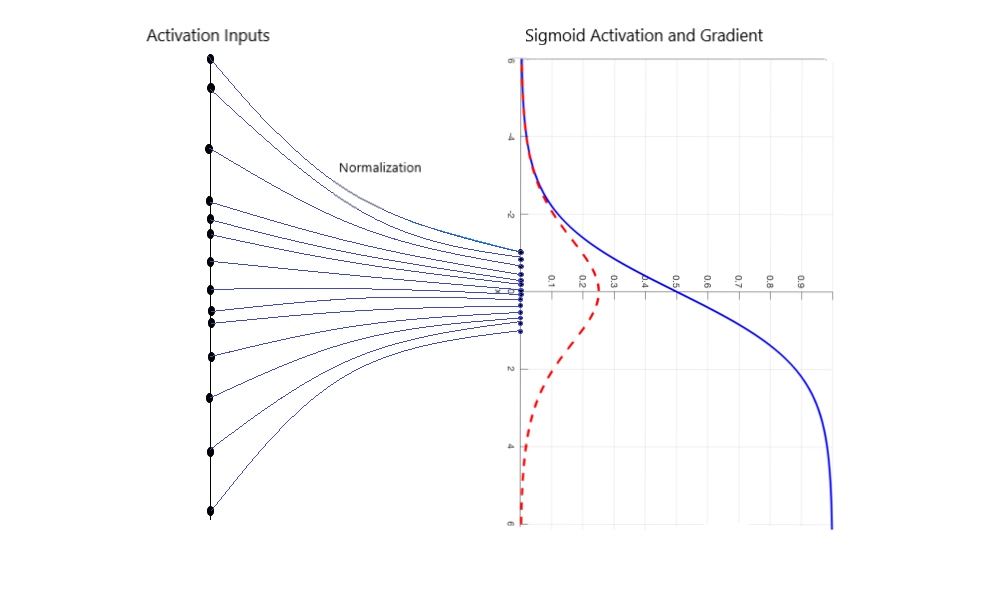
\includegraphics[width=\textwidth, trim=145 50 145 0, clip]{figures/neural_networks/batch_norm.png}
        \caption[]{Batch normalization's effect, for a single neuron, on inputs to a Sigmoid activation function.}\label{fig:batchnorm1}
    \end{subfigure}

    \begin{subfigure}[b]{0.49\textwidth}
        \centering
        \begin{tikzpicture}[
            start chain=going below, node distance=12pt,
            point/.append style={on chain, join=by {signal}},
            layer/.append style={on chain, join=by {signal}},
        ]
        \node[point] {Input};
        \node[point] {$\LARGE \vdots$};
        \node[conv] {Conv};
        \node[bn] {BatchNorm};
        \node[activation] {Sigmoid};
        \node[point] {$\LARGE \vdots$};
        \node[point] {Output};
    \end{tikzpicture}
    \caption[]{Batch normalization as a layer in a DNN.}\label{fig:batchnorm2}
    \end{subfigure}
    \caption[]{Batch normalization.}\label{fig:batchnorm}
\end{figure}